\documentclass[11pt,a4paper]{scrartcl}
\usepackage[utf8]{inputenc}
\usepackage[T1]{fontenc}
\usepackage[english]{babel}
\usepackage[babel,german=quotes]{csquotes}
\usepackage[pdftex]{graphicx}
\usepackage{amsmath,amssymb,amsthm}
\usepackage{latexsym}
\usepackage{hyperref}

\hypersetup{
pdftitle={CNN for plot function detection},
pdfsubject={Applied Machine Learning Group Project},
pdfauthor={Philipp Fürst},
pdfkeywords={wissenschaftliches Schreiben}
}
\usepackage[anythingbreaks]{breakurl}
\usepackage{listings}
\lstset{numbers=left,
	numberstyle=\small,
	numbersep=5pt,
	breaklines=true,
	showstringspaces=false,
	frame=1 ,
	xleftmargin=15pt,
	xrightmargin=15pt,
	basicstyle=\ttfamily\scriptsize,
	stepnumber=1,
	keywordstyle=\color{ao}\textbf,         
  	commentstyle=\color{gray},       
  	stringstyle=\color{mauve}         
}
\lstloadlanguages{TeX}

\usepackage{color}
\definecolor{ao}{rgb}{0.0,0.0,1.0}
\definecolor{dkgreen}{rgb}{0,0.6,0}
\definecolor{gray}{rgb}{0.5,0.5,0.5}
\definecolor{lightgray}{rgb}{0.8,0.8,0.8}
\definecolor{mauve}{rgb}{0.58,0,0.82}

\usepackage[backend=biber]{biblatex} 
\ExecuteBibliographyOptions{
sorting=nyt, 
bibwarn=true, 
isbn=false, 
url=false 
}
\addbibresource{literatur.bib} 

\setlength{\topmargin}{-10mm}

\begin{document}
\lstset{language=tex}
  \pagestyle{empty}

  \begin{titlepage}
    
    \center
    
\includegraphics[scale=0.3]{unistuttgart_logo_de} 
    \vspace*{2cm} 

 \begin{center} \large 
        
    \vspace*{2cm}

    {\huge \textbf{CNN for plot function detection}}
    \vspace*{2.5cm}

    Applied Machine Learning Group Project
    \vspace*{2.5cm}

    Philipp Fürst (3383656)\\
    Wasim Essbai (3649361)
    \vspace*{1cm}

  \end{center}
\end{titlepage}

  \tableofcontents
  
\newpage

  \pagestyle{plain}
  
  
\section{General Idea}
The aim of this group project is to use machine learning to evaluate a plot of a mathematical unknown function in order to find out the basic mathematical equation underlying its graph.
The basic problem is the classification of images. A common method for solving this type of problem is provided by the Convolutional Neural Network (CNN). 
\begin{figure}[h!]
	\centering
	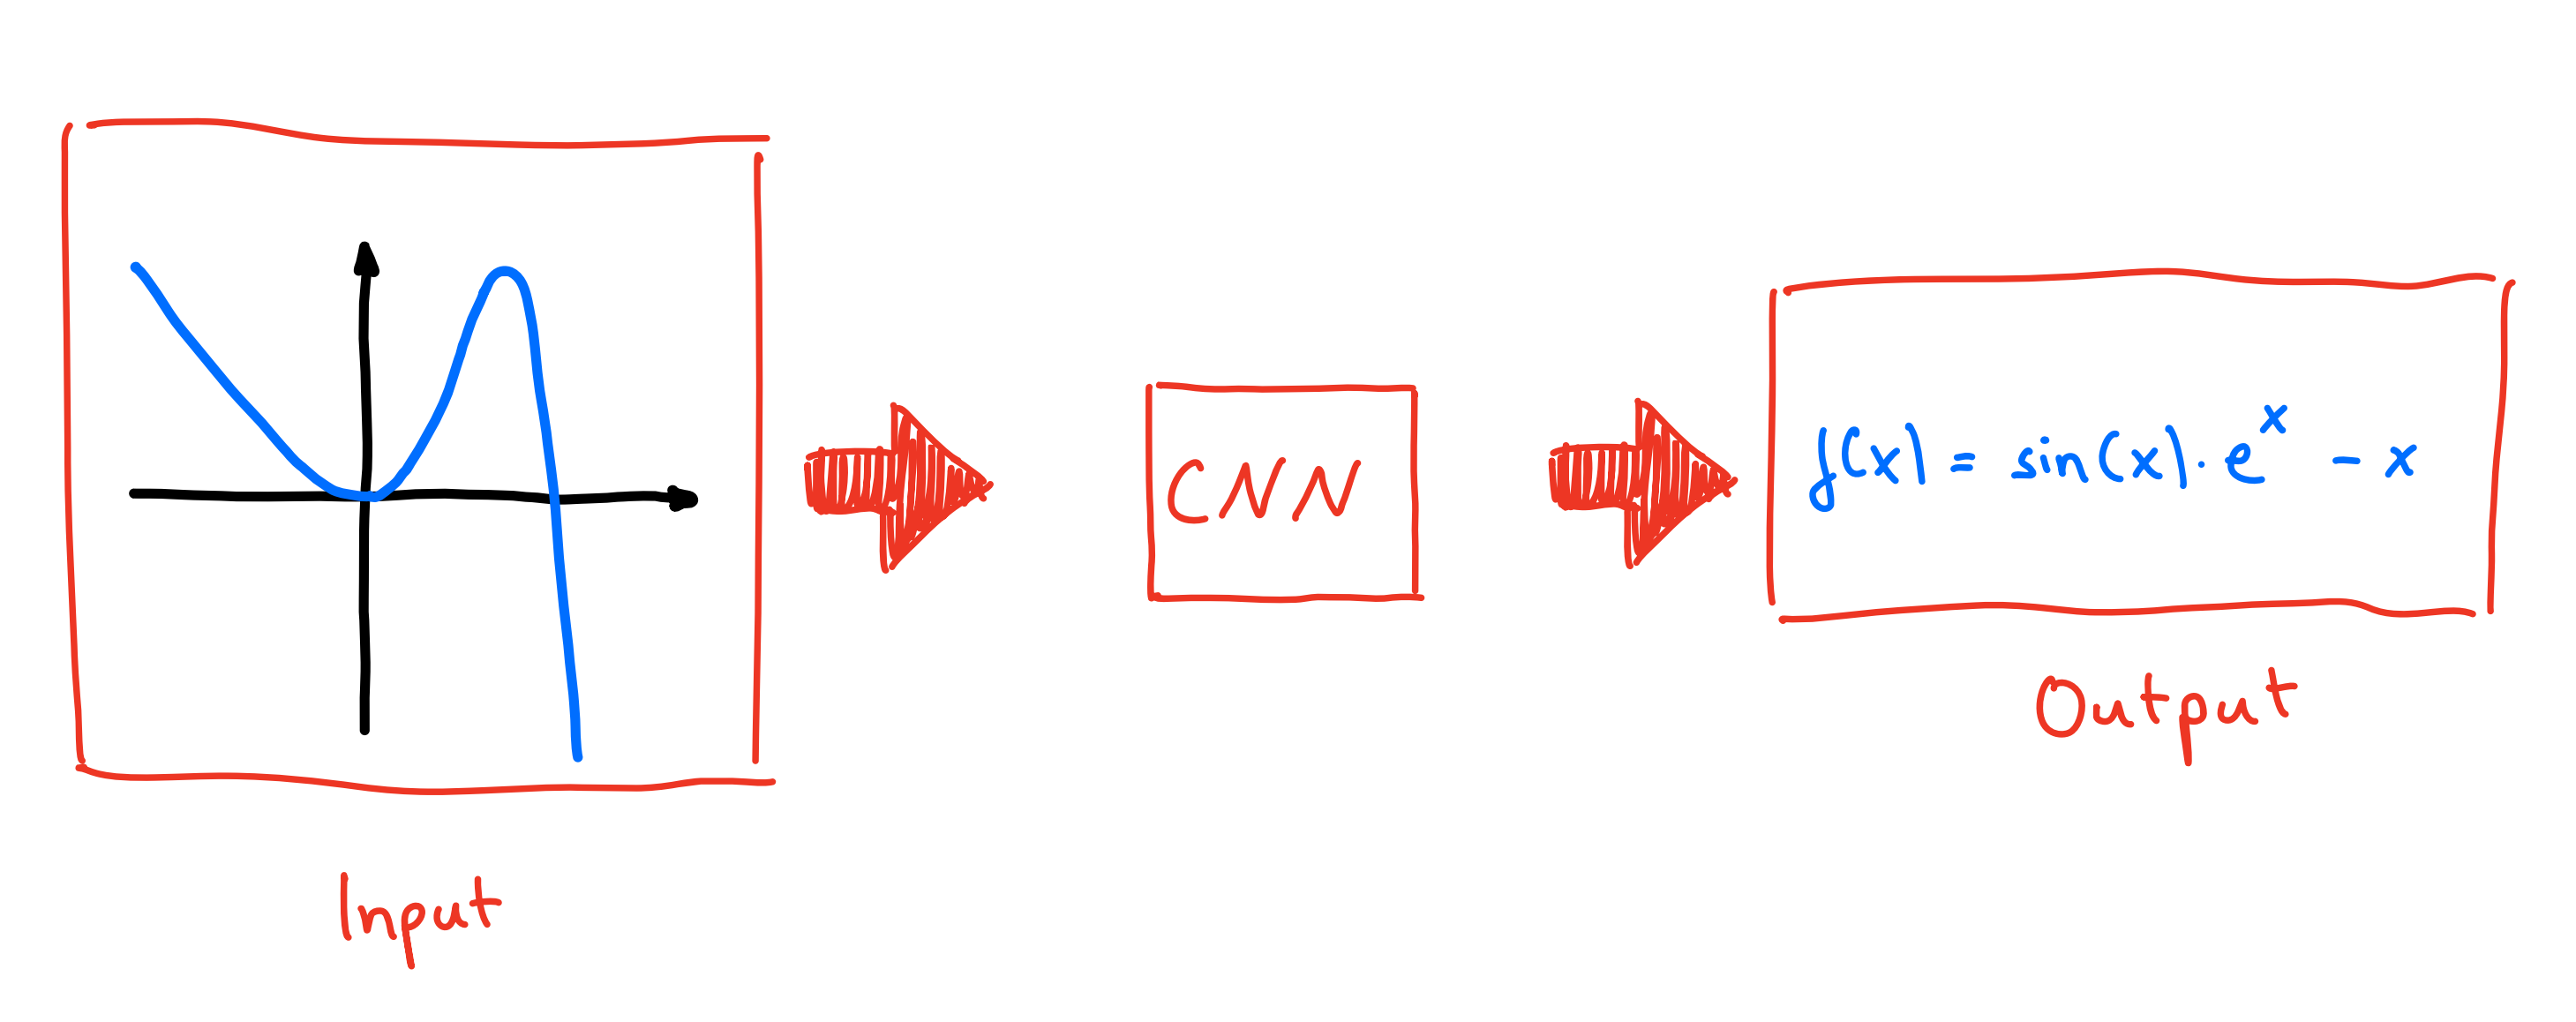
\includegraphics[width=10cm]{general_idea}
	\label{img:general_idea}
\end{figure}

\section{Data Generation}
To generate the data, we created our own code. Since there are infinite possibilities to generate functions, we limited our selection to a few basic mathematical functions, as well as the basic operators.\\
\begin{center}
	\begin{tabular}{c|c}
  		\textbf{basic function} & \textbf{basic operator}\\
  		\hline
  		\( 1 \) & \(a+b \) \\
  		\( \exp(x) \) & \(a-b \) \\
  		\( \sin(x) \) & \(a \cdot b \) \\
  		\( x^2 \) & \(a \div b \) \\
  		\( \tan(x) \) & \( a^b \) \\
  		\( \log(x) \) \\
  		\( |x| \) \\
  		\( a \)\\
  		\( x \) \\
	\end{tabular}
\end{center}
\vspace*{0.5cm}
Based on these basic functions and basic operators, we generated functions of different complexity levels. We limited our complexity level to a maximum of 3. \\
Here are some examples for different complexity levels. \\
complexity level 1:
\begin{itemize}
 \item \(f(x) = \sin(x)+x\)  
 \item \(f(x) = \log(\sin(x))\) 
 \item \(f(x) = \exp(x)/x^2\)
\end{itemize}
complexity level 2:
\begin{itemize}
 \item \(f(x) = \tan(\sin(x)+x)\)  
 \item \(f(x) = \log(\sin(x) \cdot x^2)\) 
 \item \(f(x) = |\exp(x)/\sin(x)|\)
\end{itemize}
complexity level 3:
\begin{itemize}
 \item \(f(x) = \tan(\sin(x)+x) \cdot x^2\)  
 \item \(f(x) = \log(\sin(x) \cdot a) / x\) 
 \item \(f(x) = |\exp(x)/x-a/x|\)
\end{itemize}
In addition, we divided our data set, consisting of 50000 functions/plots, into 10\% of complexity level 1, 30\% of complexity level 2 and 60\% of complexity level 3.

\subsection{Plots}
The plots form the input to the Convolutional Neural Network. The mathematical functions are always mapped in the same frame conditions. Therefore all functions are plotted in the interval \(x \in [-8,8]\), the y-axis is automatically scaled to the corresponding function values, so that relevant data is not cut off. Each plot is generated as a fixed size image (250 x 100 pixel) and read in by the CNN. The axes, as well as the grid, are removed within the plot because they are scaled differently depending on the function. Their removal creates a uniform basis and reduces the dimension of the input space, since the CNN does not have to learn this additionally. An actual input to the CNN of a function randomly selected from the dataset \(f(x) = \sin(x)+|x|\) is shown in the following plot.
\begin{figure}[h!]
	\centering
	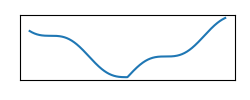
\includegraphics[width=7cm]{function_example}
	\label{img:function_example}
\end{figure}

\subsection{Labeling}
In order to be able to classify mathematical functions unambiguously by means of CNN, it is necessary to label them correctly and without loss of information. A suitable method for this is the Polish notation. We use it by assigning a numerical value to each basis function and each basis operator in order to be able to express the mathematical functions as vectors.\\
\begin{center}
	\begin{tabular}{c|c}
  		\textbf{mathematical part of function} & \textbf{corresponding label}\\
  		\hline
  		\(a+b \) & 0 \\
  		\(a-b \) & 1 \\
 		\(a \div b \) & 2 \\
  	    \(a \cdot b \) & 3 \\
  	    \( a^b \) & 4 \\
  	    \( a \) & 5 \\
  	    \( x \) & 6 \\
  		\( 1 \) & 7 \\
  		\( \exp(x) \) & 8 \\
  		\( \sin(x) \) & 9 \\
  		\( x^2 \) & 10 \\
  		\( \tan(x) \) & 11 \\
  		\( \log(x) \) & 12\\
  		\( |x| \) &13 \\
	\end{tabular}
\end{center}
\vspace*{0.5cm}
Each vector has a maximum length of 15, which is reached when complexity level 3 is executed with the maximum number of binary operators. All functions which are less complex and therefore would create a vector with fewer entries are stretched to the length of 15 by simply executing the identity function. This becomes recognizable by the combination sequence of 6 and 7 towards the end of the vector, because an execution of the identity function corresponds to a simple multiplication by 1. This does not change the actual function, however, thereby it is reached that all vectors possess 15 entries. Each entry itself can take the numerical values between 0 and 13. The following is an example of such a labeling.\\
\begin{center}
	\(f(x) = \sin(x)+|x|\) \\
	$\Downarrow$ \\ 
	\(x,1,x,1,x,1,x,1,x,1,x,1,+,sin(x),|x|\)\\
	$\Downarrow$ \\ 
	\( (13,9,0,7,6,7,6,7,6,7,6,7,6,7,6) \)\\
\end{center}

\section{CNN model}
Our CNN has the following structure.
\begin{lstlisting}
 class FrCNet(Module):
    def __init__(self, numChannels, output_size):
        super(FrCNet, self).__init__()
        self.network = Sequential(

            Conv2d(numChannels, 16, kernel_size=2, padding=1),
            ReLU(),
            MaxPool2d(2, 2),

            Conv2d(16, 32, kernel_size=2, padding=1),
            ReLU(),
            MaxPool2d(2, 2),

            Conv2d(32, 64, kernel_size=2, padding=0),
            ReLU(),
            MaxPool2d(2, 2),

            Flatten(),
            Linear(23808, 1012),
            ReLU(),
            Linear(1012, 512),
            ReLU(),
            Linear(512, output_size),
        )
\end{lstlisting}
\textcolor{red}{Put in graphic of our CNN}

\section{Training}
First we created a smaller data set consisting of 2000 function plots and the corresponding function vectors. This was again split into 70\% training data, 15\% validation data and 15\% test data. Based on this we tested different sizes of kernels, epochs and learning rates, as there the execution time remained manageable.\\
\\
We achieved the highest performance with 2x2 kernels, padding of the first two convolutional layers, 15 epochs, 0.1\% learning rate, and a scaling factor of 1000000, which further separates the closely spaced numbers of vector entries, allowing easier learning of the entries.\\
 \\
With these parameters found, we could train the CNN on our large dataset (50000). The execution of the training was done GPU-based on Google Colab.
\section{Experimental Results}
\textcolor{red}{learning curve of loss over epochs and accuracy over epochs, for full vector length and not full vector length (both on the big data set)}
\section{Conclusion}
Our general idea works. It is possible to recognize functions from a given plot and to classify their mathematical function using our trained CNN. The performance is still improvable. \\
\\
Among other things, this is due to the fact that there are redundancies within our data sets, which are currently not filtered out. For example, one and the same function can be generated by different mathematical functions \(f(x) = |x^2| = x^2\). Eliminating these would be a first step to have a more meaningful dataset. \\
\\
Additionally, due to lack of computer resources, we trained our CNN on only 50000 samples. This is very small in the dimension of machine learning and therefore still expandable. However, the approach is promising if already with these small data sets accuracies of \textcolor{red}{X.XX\%} are achieved when comparing all but one vector entries of the mathematical function. 

\end{document}